\section{Casos de uso}
A continuación se detalla el modelado de las entidades de negocio y su funcionalidad dentro de la aplicación, así mismo su interacción con los actores que intervendrán en la aplicación.\par
\vspace{5mm}
\begin{enumerate}[1.]
\item Login

\subsection{Login}
\begin{figure}[h!]
	\centering
	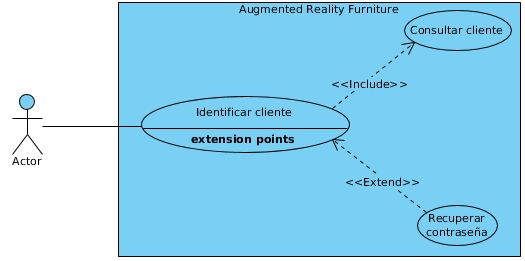
\includegraphics[width=7cm,height=7cm]{imagenes/analisis/login.jpg}
	\caption{CU01 Login.\cite{B27}}
	\label{fig:analogo}
\end{figure}  
\newpage
\item Registrar usuario
\subsection{Registrar usuario} 
\begin{figure}[h!]
	\centering
	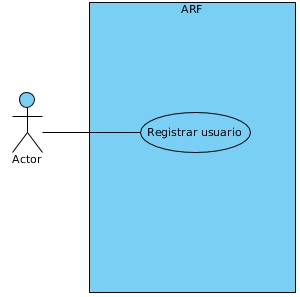
\includegraphics[width=7cm,height=7cm]{imagenes/analisis/registrarUsuario.jpg}
	\caption{CU02 Registrar un usuario.\cite{B27}}
	\label{fig:analogo}
\end{figure} 
\item Recuperar contraseña
\subsection{Recuperar contraseña} 
\begin{figure}[h!]
	\centering
	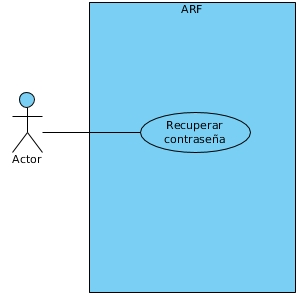
\includegraphics[width=7cm,height=7cm]{imagenes/analisis/recuperarContrasenia.jpg}
	\caption{CU3 Recuperar contrasenia.\cite{B27}}
	\label{fig:analogo}
\end{figure}
\item Gestion de escenario
\subsection{Gestión de escenario} 
\begin{figure}[h!]
	\centering
	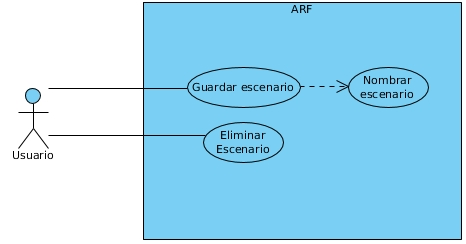
\includegraphics[width=6cm,height=6cm]{imagenes/analisis/Escenario.jpg}
	\caption{CU04 Gestionar escenarios\cite{B27}}
	\label{fig:analogo}
\end{figure}

\item Visualizacion de escenario
\subsection{Visualización de escenario} 
\begin{figure}[h!]
	\centering
	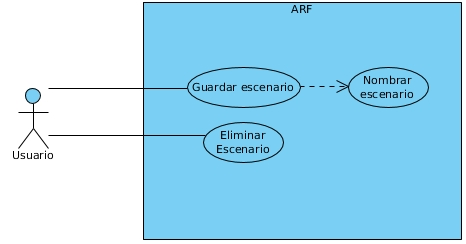
\includegraphics[width=7cm,height=7cm]{imagenes/analisis/Escenario.jpg}
	\caption{Visualizacion de escenario \cite{B27}}
	\label{fig:analogo}
\end{figure}
\end{enumerate}

